%%
%% lec6.tex
%% 
%% Made by Patrick E. McKnight
%% Login   <pem@copernicus>
%% 
%% Started on  Fri Mar 14 06:40:26 2008 Patrick E. McKnight
%% Last update Mon Mar  1 18:23:13 2010 Patrick McKnight
%%
\documentclass[12pt]{article}
% \usepackage{savetrees}
\usepackage{tikz}
\usetikzlibrary{positioning,shadows,arrows,fit,backgrounds,calc}
\usepackage{latexsym}
\usepackage[text={7in,9.5in},centering]{geometry}
\usepackage{graphicx}
\usepackage{mdwlist}
%\usepackage[usenames]{color}
%\usepackage{wrapfig}
\usepackage[utf8]{inputenc}
\usepackage[T1]{fontenc}
%\usepackage[thinlines]{easytable}
\usepackage{longtable}
\usepackage{float}
%\usepackage{pdfpages}
\title{PSYC 612, SPRING 2012\\Introduction to Mediation}
\date{Lecture Week: 2/14/2012}

\newcommand{\squishlist}{
   \begin{list}{$\bullet$}
    { \setlength{\itemsep}{0pt}      \setlength{\parsep}{3pt}
      \setlength{\topsep}{3pt}       \setlength{\partopsep}{0pt}
      \setlength{\leftmargin}{1.5em} \setlength{\labelwidth}{1em}
      \setlength{\labelsep}{0.5em} } }

\newcommand{\squishlisttwo}{
   \begin{list}{$\rhd$}
    { \setlength{\itemsep}{0pt}    \setlength{\parsep}{0pt}
      \setlength{\topsep}{0pt}     \setlength{\partopsep}{0pt}
      \setlength{\leftmargin}{2em} \setlength{\labelwidth}{1.5em}
      \setlength{\labelsep}{0.5em} } }

\newcommand{\squishlistthree}{
   \begin{list}{$-$}
    { \setlength{\itemsep}{0pt}    \setlength{\parsep}{0pt}
      \setlength{\topsep}{0pt}     \setlength{\partopsep}{0pt}
      \setlength{\leftmargin}{2.5em} \setlength{\labelwidth}{2em}
      \setlength{\labelsep}{0.5em} } }

\newcommand{\squishend}{
    \end{list}  }

\newcommand{\callout}[1]{
 \begin{center}
 \begin{tikzpicture}[thick]
 \tikzstyle{txt} = [fill=yellow!10,shape=rectangle,text width=5in]
 \tikzstyle{bgy} =  [fill=yellow!10,thick,draw=black,rounded corners=2mm]
 \node[txt] (qu) at (0,0)  {#1} ;
 \begin{pgfonlayer}{background}
 \node[bgy] (background) [fit = (qu)] {};
 \end{pgfonlayer}
 \end{tikzpicture}
 \end{center}
}

\newcommand{\eqncallout}[1]{
 \begin{center}
 \begin{tikzpicture}[thick]
 \tikzstyle{eqn} = [fill=blue!10,shape=rectangle]
 \tikzstyle{bgb} =  [fill=blue!10,thick,draw=black,rounded corners=2mm]
 \node[eqn] (qu) at (0,0)  {#1} ;
 \begin{pgfonlayer}{background}
 \node[bgb] (background) [fit = (qu)] {};
 \end{pgfonlayer}
 \end{tikzpicture}
 \end{center}
}

  
  
\usepackage{Sweave}
\begin{document}
\input{612Med1-concordance}
\maketitle
\tableofcontents

\hrulefill

\section{Preliminary Questions}

\squishlist
\item How are the modules going?
\item Did you read the Iacobucci text?
\squishend

\section{Part I: Preview of Mediation and Moderation  (30 minutes; 2 minute break)}

\hrulefill
\subsection{Purpose:} Provide you with the necessary background
information about the topics mediation and moderation

\subsection{Objectives:}

\begin{enumerate*}
\item Introduce mediation
\item Introduce moderation and contrast it with mediation
\end{enumerate*}
\hrulefill

\subsection{Mediation}

Mediation is best explained graphically. We begin with a simple path
diagram - note the similarity to my advance organizer?

\pgfdeclarelayer{background}
\pgfdeclarelayer{foreground}
\pgfsetlayers{background,main,foreground}
%% Bivariate model
\begin{center}
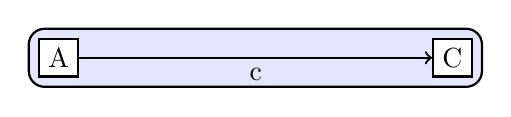
\begin{tikzpicture}[thick]
\tikzstyle{mv} = [draw,fill=white,shape=rectangle]
\tikzstyle{lv} = [draw,fill=white,shape=circle]
\tikzstyle{bgb} = [fill=blue!10,thick,draw=black,rounded corners=2mm]
\tikzstyle{bgy} =  [fill=yellow!10,thick,draw=black,rounded corners=2mm]
\node[mv] (A) at (0,0)  {A} ;
\node[mv] (C) at (5,0)  {C} ;
\draw [->] (A) -- (C)  node [midway,below,draw=none] {c} ;
\begin{pgfonlayer}{background}
\node[bgb] (background) [fit = (A) (C)] {};
\end{pgfonlayer}
\end{tikzpicture}
\end{center}

That path model depicts a single manifest variable $A$ predicting a
single manifest variable $C$ - a bivariate relationship often
expressed as a correlation or a bivariate regression $c$.  Causal
inference gets a bit more complicated when we introduce another
variable into the fold.  Typically, we just include that additional
variable as another predictor of our oucome $c$ as depicted here:


%% Two predictor model
\begin{center}
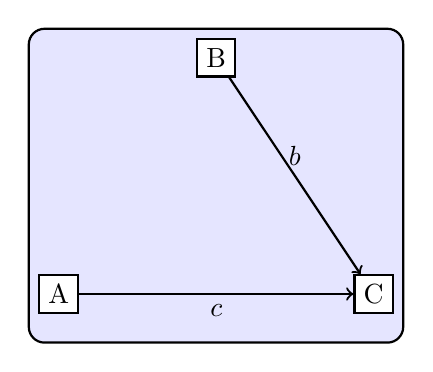
\begin{tikzpicture}[thick]
\tikzstyle{mv} = [draw,fill=white,shape=rectangle]
\tikzstyle{lv} = [draw,fill=white,shape=circle]
\tikzstyle{bgb} = [fill=blue!10,thick,draw=black,rounded corners=2mm]
\tikzstyle{bgy} =  [fill=yellow!10,thick,draw=black,rounded corners=2mm]
\coordinate (bot) at (1,-.5);
\node[mv] (A) at (1,0)  {A} ;
\node[mv] (B) at (3,3)  {B} ;
\node[mv] (C) at (5,0)  {C} ;
\draw [->] (A) -- (C)  node [midway,below,draw=none] {$c$} ;
\draw [->] (B) -- (C)  node [midway,above,draw=none] {$b$} ;
\begin{pgfonlayer}{background}
\node[bgb] (background) [fit = (A) (B) (C) (bot)] {};
\end{pgfonlayer}
\end{tikzpicture}
\end{center}


What happens when we expect a temporal relationship between our
antecedent $A$ and our consequence $C$ to be causally related to our
second predictor $B$?  A relationship like that is depicted as:

%% Mediation model
\begin{center}
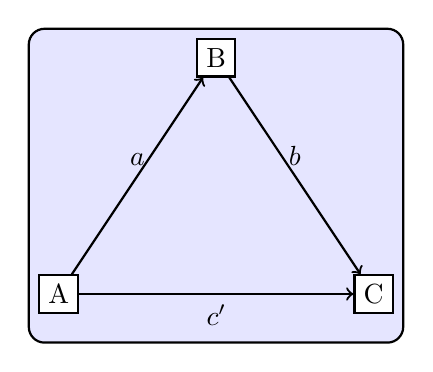
\begin{tikzpicture}[thick]
\tikzstyle{mv} = [draw,fill=white,shape=rectangle]
\tikzstyle{lv} = [draw,fill=white,shape=circle]
\tikzstyle{bgb} = [fill=blue!10,thick,draw=black,rounded corners=2mm]
\tikzstyle{bgy} =  [fill=yellow!10,thick,draw=black,rounded corners=2mm]
\coordinate (bot) at (1,-.5);
\node[mv] (A) at (1,0)  {A} ;
\node[mv] (B) at (3,3)  {B} ;
\node[mv] (C) at (5,0)  {C} ;
\draw [->] (A) -- (C)  node [midway,below,draw=none] {$c^\prime$} ;
\draw [->] (A) -- (B)  node [midway,above,draw=none] {$a$} ;
\draw [->] (B) -- (C)  node [midway,above,draw=none] {$b$} ;
\begin{pgfonlayer}{background}
\node[bgb] (background) [fit = (A) (B) (C) (bot)] {};
\end{pgfonlayer}
\end{tikzpicture}
\end{center}

The model above shows a mediation model whereby $B$ mediates (i.e.,
sits between) the antecedent $A$ and the consequence $C$.
Unfortunately, we learned that the GLM restricts us to a single
dependent variable; thus, we cannot simultaneously analyze prediction
of $C$ by $A$ and $B$ along with the prediction of $B$ by $A$.  The
solution to this problem is the basis for today's discussion -
mediation analysis.

\subsection{Moderation}

Before we get to mediation, I want to contrast mediation with
moderation.  Many of you already know about moderation because
moderation is nothing more than an interaction.  This figure shows a
moderated relationship for our three aforementioned variables:

%% Moderation model
\begin{center}
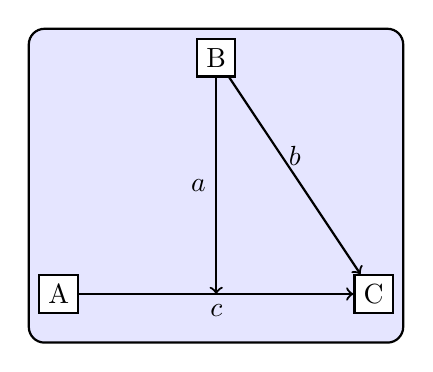
\begin{tikzpicture}[thick]
\tikzstyle{mv} = [draw,fill=white,shape=rectangle]
\tikzstyle{lv} = [draw,fill=white,shape=circle]
\tikzstyle{bgb} = [fill=blue!10,thick,draw=black,rounded corners=2mm]
\tikzstyle{bgy} =  [fill=yellow!10,thick,draw=black,rounded corners=2mm]
\coordinate (bot) at (1,-.5);
\node[mv] (A) at (1,0)  {A} ;
\node[mv] (B) at (3,3)  {B} ;
\node[mv] (C) at (5,0)  {C} ;
\draw [->] (A) -- (C)  node [midway,below,draw=none] {$c$} ;
\draw [->] (B) -- (3,0)  node [midway,left,draw=none] {$a$} ;
\draw [->] (B) -- (C)  node [midway,above,draw=none] {$b$} ;
\begin{pgfonlayer}{background}
\node[bgb] (background) [fit = (A) (B) (C) (bot)] {};
\end{pgfonlayer}
\end{tikzpicture}
\end{center}


\section{Part II: Demonstrate a Mediational Analysis (40 minutes)}

\hrulefill
\subsection{Purpose:} Solidify conceptual knowledge with an example

\subsection{Objectives:}

\begin{enumerate*}
\item Describe data and model
\item Run mediational analysis
\item Discuss results in detail
\end{enumerate*}
\hrulefill

\subsection{The Data and Mediation Model}

A recent Department of Education report on the ``Equity in Athletics''
provided us with a convenient dataset to demonstrate mediational
models.  I am only using a small portion of the data for illustrative
purposes only.  There are probably better datasets than this one but
it is current and reasonably interesting so that we can all have some
fun.  You may find the data on the MRES website; please download it if
you care to run the same models I run below.

